\chapter{Amazon Web Services (AWS)}

Amazon usluge za web \engl{Amazon Web Services - AWS} sveobuhvatna je platforma za računarstvo u oblaku koju pruža tvrtka Amazon te sadrži brojne usluge u oblaku, uključujući infrastrukturu \engl{Infrastructure as a Service - IaaS}, platformu \engl{Platform as a Service - PaaS} i softver \engl{Software as a Service - SaaS}. AWS usluge nude organizacijske alate kao što su računalna snaga, baza podataka i usluge isporuke sadržaja \cite{what_is_aws}. 

AWS je podijeljen u više različitih usluga koje se mogu pojedinačno konfigurirati na temelju korisničkih potreba. Neke od usluga koje nudi AWS su: pohrana, baze podataka, monitoriranje, sigurnost, analitika, umjetna inteligencija te razvoj mobilnih aplikacija. 

AWS pruža usluge iz mnogo podatkovnih centara \engl{data center - DC} koji su raspodijeljeni po zonama dostupnosti \engl{availability zone - AZ} diljem regija cijelog svijeta. Jedna regija obuhvaća nekoliko fizički bliskih zona povezanih mrežom niske latencije. Geografskom raspodijeljenošću AWS pruža višestruke prednosti \cite{aws_regions}:
\begin{enumerate}
	\item niska latencija: budući da su regije skupovi fizičkih mrežno povezanih bliskih zona, korisnički podaci i aplikacije mogu biti smješteni bliže krajnjim korisnicima što poboljšava performanse aplikacija,
	\item visoka dostupnost: u slučaju kvara podatkovnog centra, korištenjem više zona dostupnosti unutar regije podaci mogu i dalje ostati dostupni,
	\item otpornost i oporavak od katastrofe: podaci i aplikacije mogu se replicirati između više zona ili regija, što omogućava brzi oporavak u slučaju prirodnih katastrofa, tehničkih problema ili napada,
	\item skalabilnost: klijenti mogu dinamički povećavati ili smanjivati resurse u različitim regijama ovisno o potražnji,
	\item poboljšana sigurnost: fizički odvojeni podatkovni centri smanjuju rizik od pojedinačnih točaka neuspjeha i omogućavaju implementaciju složenijih sigurnosnih strategija.
\end{enumerate}

Također, nude se brojne mogućnosti za razvojne inženjere u sklopu AWS-a. Nudi alate naredbenog retka \engl{command-line tools} i pakete za razvoj programa \engl{Software Development Kit - SDK} za puštanje aplikacija u produkciju \engl{deployment} i upravljanje vlastitim uslugama i aplikacijama. Paketi za razvoj programa dostupni su u raznim programskim jezicima, uključujući programske jezike C++, Android, iOS, Java, Node.js, Python i Ruby.

AWS isto tako nudi brojne usluge za razvoj IoT sustava. Usluga AWS-a za IoT pruža platformu za upravljanje IoT uređajima te obradu podataka i njihovu pohranu na druge AWS usluge, poput baze podataka. AWS IoT pruža usluge u oblaku koje povezuju IoT uređaje s drugim uređajima i uslugama AWS-a u oblaku. Također pruža softver za uređaje, poput paketa za razvoj programa, za jednostavniju integraciju s uslugama AWS-a za IoT. Na slici \ref{fig:aws_iot_arch} nalazi se prikaz arhitekture usluga koje AWS nudi za razvoj IoT sustava.

\begin{figure}[ht]
	\centering
	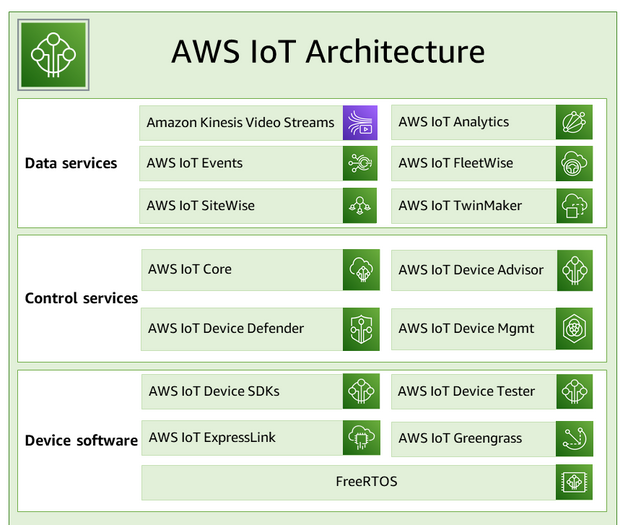
\includegraphics[scale=0.8]{imgs/aws_iot_arch}
	\caption{Arhitektura usluga AWS-a za IoT \cite{aws_docs}}
	\label{fig:aws_iot_arch}
\end{figure}

AWS podržava sljedeće komunikacijske protokole za IoT sustave:
\begin{itemize}
	\item MQTT \engl{Message Queuing Telemetry Transport},
	\item HTTPS,
	\item LoRaWAN \engl{Long Range Wide Area Network},
	\item TLS.
\end{itemize}

U nastavku su opisane usluge koje nudi AWS za razvoj IoT sustava.

\section{AWS IoT Core}

AWS IoT Core ključna je komponenta za integraciju oblaka i fizičkih uređaja. Omogućava povezivanje uređaja i preusmjeravanje poruka na usluge AWS-a. Koristi MQTT koji je standardni protokol za razmjenu poruka u IoT sustavima. To je lagan \engl{lightweight} protokol za prijenos poruka temeljen na objavi/pretplati sustavu u kojoj glavnu ulogu ima broker kao posrednik, te je pogodan za povezivanje udaljenih uređaja uz minimalnu potrošnju \cite{what_is_mqtt}. AWS IoT Core pruža paletu značajki za razmjenu poruka temeljenih na protokolu MQTT, koje pomažu pri izradi prilagodljive i skalabilne IoT arhitekture \cite{aws_docs}. Komponenta također ima ugrađenu podršku za upravljanje MQTT brokerom koji podržava trajne, uvijek uključene veze, napredna pravila zadržavanja poruka te obrađuje više uređaja i tema istovremeno. Isto tako, AWS IoT Core podržava najnoviji standard MQTT 5 i kompatibilan je sa prethodnim standardom MQTT 3, što omogućuje učinkovito upravljanje heterogenim implementacijama s mnoštvom specifikacija. Nadalje, komponenta omogućava višestruke metode provjere autentičnosti i pristupne politike za zaštitu rješenja od ranjivosti. Štoviše, koristeći pomoć drugih usluga u sklopu platforme kao što je AWS IoT Core Device Advisor, moguće je pristupiti unaprijed izgrađenim paketima testova za provjeru MQTT funkcionalnosti uređaja tijekom faze razvoja.

Na slici \ref{fig:aws_iot_core_overview} nalazi se pregled rada usluge AWS IoT Core.

\begin{figure}[ht]
	\centering
	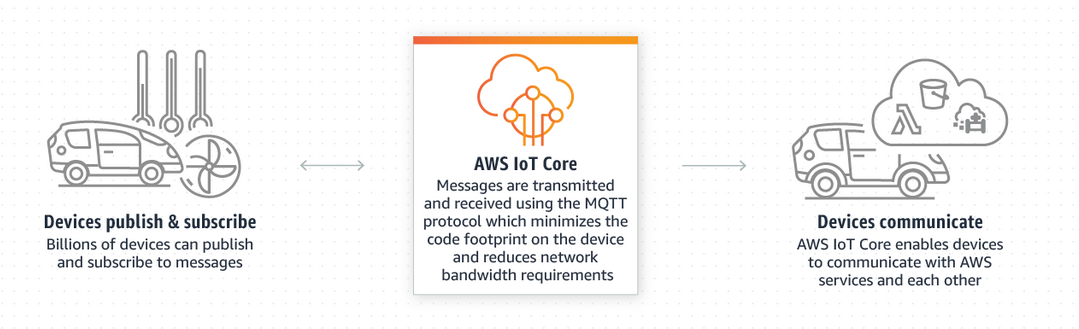
\includegraphics[scale=0.6]{imgs/aws_iot_core_overview}
	\caption{Princip rada usluge AWS IoT Core \cite{aws_docs}}
	\label{fig:aws_iot_core_overview}
\end{figure}

AWS IoT Core pruža usluge koje povezuju oblak AWS-a s IoT uređajima kako bi se ostale usluge u oblaku i aplikacije mogle međusobno komunicirati s tim uređajima. Na slici \ref{fig:aws_iot_core_components} nalaze se svi segmenti usluge AWS IoT Core te kako oni komuniciraju s vanjskim dijelovima. Zelenom bojom označena je sama usluga, narančastom bojom fizički uređaji odnosno stvari (engl. \textit{Things}), sivom bojom druge IoT aplikacije unutar AWS-a koje se mogu izravno spojiti na sustave u AWS-u, dok su plavom bojom označene ostale usluge odnosno sustavi koji se nalaze u ekosustavu AWS.

\begin{figure}[ht]
	\centering
	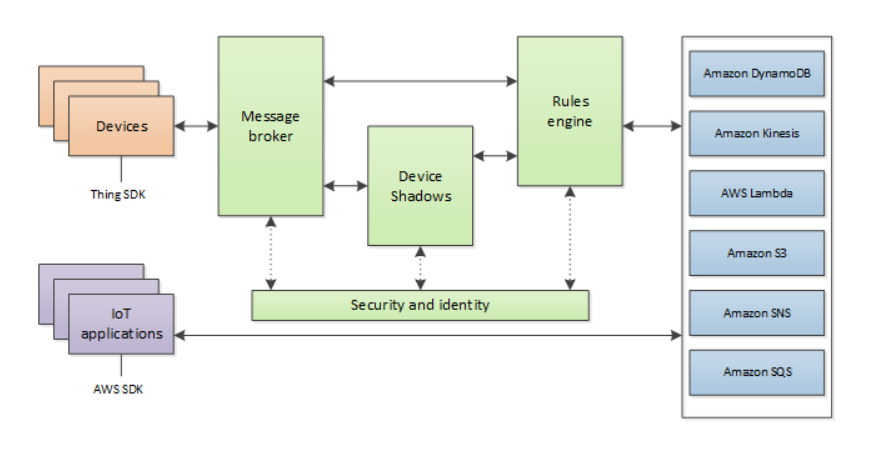
\includegraphics[scale=0.6]{imgs/aws_iot_core_components}
	\caption{Komponente usluge AWS IoT Core \cite{aws_docs}}
	\label{fig:aws_iot_core_components}
\end{figure}

U nastavku su ukratko opisane ključne usluge koje pokriva AWS IoT Core \cite{aws_docs}.

\subsubsection{Usluge za slanje poruka}

AWS IoT Core usluge za povezivanje pružaju sigurnu komunikaciju s IoT uređajima i upravlja porukama koje prolaze između uređaja i oblaka.

Prilazni uređaj omogućuje uređajima sigurnu i efikasnu komunikaciju sa sustavom AWS. Komunikacija je osigurana sigurnosnim protokolima koji koriste  X.509 certifikate. 

Broker za poruke pruža mehanizam uređajima i aplikacijama slanje i primanje poruka. Moguće je koristiti protokol MQTT ili direktno \textit{WebSocket} za objavu i pretplatu na teme. Uređaji i klijenti koriste sučelje HTTP REST za objavu poruka brokeru. Broker zatim distribuira podatke na uređaje koji su se pretplatili na određene teme kao i na druge AWS aplikacije te usluge koje prate teme na brokeru.

AWS IoT Core za protokol LoRaWAN omogućava postavljanje privatne LoRaWAN mreže tako što poveže LoRaWAN te prilazne uređaje na AWS bez potrebe za razvojem mrežnog servera za LoRaWAN \engl{LoRaWAN Network Server - LNS}. Poruke primljene od LoRaWAN uređaja šalju se na stroj za pravila \engl{rules engine} gdje se formatiraju i prosljeđuju ostalim AWS uslugama.

Stroj za pravila \engl{rules engine} povezuje podatke iz brokera s drugim AWS IoT uslugama za pohranu i dodatnu obradu. Primjerice, moguće je umetati ili pretraživati po podatkovnim tablicama ili pozvati određene definirane funkcije na temelju izraza definiranog u stroju. Isto tako, moguće je obraditi te podatke i proslijediti novostvoreni format poruka drugim uslugama ili bazama podataka.

\subsubsection{Upravljačke usluge}

Upravljačke usluge AWS IoT Core komponente pružaju sigurnost uređaja te značajke za upravljanje i registraciju novih uređaja.

Moguće je definirati vlastite autorizatore radi upravljanja autentifikacijskim i autorizacijskim strategijama koristeći vlastiti servis za autentifikaciju i funkcije za računanje Lambda koje nudi AWS. Lambda je računalna usluga za slučajeve i aplikacije dinamičke skalabilnosti. Pokreće kod na infrastrukturi visoke dostupnosti i obavlja cjelokupnu administraciju računalnih resursa, uključujući održavanje poslužitelja i operativnog sustava, osiguravanje kapaciteta i automatsko skaliranje ovisno o trenutnim potrebama sustava. Lambda funkcije korisne su za obradu datoteka, tokova te HTTP zahtjeva. Funkcije su pogodne za obradu podataka prije preusmjeravanja na drugu funkciju ili pohranu. 

Usluga za registraciju uređaja u sustav \engl{provisioning} omogućava konfiguriranje i prijavu uređaja u AWS koristeći predložak koji opisuje resurse potrebne uređaju: stvar, certifikat i nekoliko politika. Stvar \engl{thing} je unos u registar koji sadrži atribute opisa uređaja. Uređaji koriste certifikate za autentifikaciju sa sustavom AWS. Politike određuju koje operacije uređaj može izvršiti. Svaka politika ima definirani dokument s izjavom koja se sastoji od učinka, akcije i resursa nad kojim se akcija izvršava. Učinak može biti \textit{Dopusti} ili \textit{Uskrati}, akcija se odnosi nad radnje s MQTT brokerom i poslovima, a resurs se odnosi na regiju i račun u kojem politika vrijedi. 

Isto tako, moguće je definirati grupe za lakšu kategorizaciju i upravljanje uređajima. Grupe također mogu imati podgrupe, i tako graditi hijerarhiju grupa. Sve akcije izvršene na roditeljima propagiraju se do najdubljih podgrupa. Dozvole dodijeljene grupi primjenjuju se na sve uređaje u toj grupi i svim njihovim podgrupama. 

Usluga za poslove \engl{jobs} omogućava definiranje udaljenih operacija koje se pošalju i izvrše na fizičkim uređajima spojenih u oblak. Posao se može odnositi preuzimanje i instalaciju aplikacija, ažuriranje sustava, ponovno pokretanje, obnova certifikata i slično.

Usluga za sigurnost i identitet pruža dijeljenu odgovornost za sigurnost unutar AWS oblaka. Fizički uređaji moraju držati vjerodajnice na sigurnom kako bi se podaci mogli slati brokeru na siguran način. Značajke za sigurnost koriste i stroj za pravila kao i broker za poruke radi sigurnog prijenosa podataka drugim uslugama unutar AWS ekosustava.

\subsubsection{Usluge za uređaje}

AWS IoT Core osigurava pouzdano aplikacijsko iskustvo iako uređaji nisu uvijek povezani. 

Sjena uređaja \engl{Device Shadow} dokument je u JSON formatu koji se koristi za pohranu i dohvat trenutnog stanja i informacija o uređaju. AWS nudi uslugu koja održava stanje uređaja \engl{Device Shadow service} kako bi aplikacije mogle komunicirati s uređajem bez obzira je li uređaj na mreži ili ne. Kada uređaj nije priključen na mrežu, usluga sjene uređaja upravlja podacima za povezane uređaje. Kada se uređaj ponovno spoji na mrežu, sinkronizira stanje sa sjenom uređaja koja se nalazi u oblaku. Uređaji također mogu objavi svoje stanje usluzi u bilo kojem trenutku kako bi bilo na raspolaganju drugim aplikacijama i uređajima. 

\subsection{AWS IoT Fleet Provisioning}

Kao što je ranije navedeno, AWS nudi uslugu registracije uređaja u sustav čime uređaj dobiva pristup ostalim uslugama unutar platforme, poput povezivanja na MQTT broker. Moguće je dinamički registrirati više uređaja pomoću privremenih ili trajnih certifikata, što se naziva provizioniranje flote \engl{fleet provisioning}. Pomoću ove usluge AWS generira i sigurno dostavi certifikate te privatne ključeve na uređaje pri prvom povezivanju na platformu. AWS izdaje klijentske certifikate koji su potpisani certifikacijskim tijelom tvrtke Amazon \engl{Certificate Authority - CA} \cite{aws_docs}.

Tri su ključna koraka pri omogućavanju registracije više uređaja u sustav:
\begin{enumerate}
	\item određivanje načina registracije,
	\item definiranje upravljačke strukture nad uređajima,
	\item kreiranje predloška za registraciju.
\end{enumerate}

Određivanje načina registracije u sustav povezano je s odabirom vrste certificiranja koja će se koristiti. Uređaji trebaju jedinstveni certifikat za povezivanje s platformom AWS i korištenje njenih usluga. Postoje tri metode certificiranja uređaja te odabir ovisi o mogućnostima proizvodnje uređaja i ovlastima samih korisnika:
\begin{itemize}
	\item registracija uređaja vlastitim jedinstvenim certifikatima, 
	\item registracija od strane korisnika od povjerenja,
	\item registracija certifikatom zahtjeva.  
\end{itemize} 

Registracija uređaja vlastitim jedinstvenim certifikatima podrazumijeva postojanje verificiranih certifikata na samom uređaju pri prvom povezivanju u sustav. Ovaj se način još naziva i pravodobno provizioniranje \engl{just-in-time provisioning}. Problem s ovim pristupom jest što instalacija certifikata nije uvijek moguća prije dostave uređaja korisniku. Isto tako, čak iako je instalacija certifikata moguća, nije uvijek moguće instalirati certifikate sigurno na uređaj, stoga je potrebno koristiti alternativne metode. 

U slučaju kada rana certifikacija uređaja nije moguća, autorizirani ili krajnji korisnici \engl{trusted users} mogu uz pomoć aplikacije registrirati uređaje prije njihova spajanja na platformu. Ovdje je potrebno korisnicima pružiti aplikaciju kojom bi konfigurirali uređaj prilikom instalacije, te \textit{firmware} uređaja mora podržavati ovaj način registracije. 

Treća opcija jest registracija pomoću certifikata zahtjeva \engl{claim certificate}. Certifikati zahtjeva privremeni su certifikati koji se mogu instalirati na više uređaja, te se pri prvoj registraciji u sustav zamijene s novim, jedinstvenim certifikatom. Ova metoda zahtijeva dodatne sigurnosne provjere zbog mogućnosti curenja privremenih certifikata zahtjeva jer više uređaja dijeli isti certifikat, no prijetnja se može ublažiti redovitim rotiranjem privremenih certifikata te kreiranjem više certifikata zahtjeva koji se mogu koristiti. Isto tako, privremenim certifikatima potrebno je dodijeliti minimalan skup dozvoljenih radnji potrebnih za registraciju uređaja. Dodatna sigurnosna provjera može se izvršiti i u obliku Lambda funkcije dodatnom provjerom primljenih parametara s uređaja.

Upravljačka struktura nad uređajima je važna radi lakše organizacije uređaja u samom sustavu. Povezani uređaji predstavljeni su u platformi kao stvari tj. resursi koji se mogu organizirati i održavati. Osim ranije spomenutih stvari i grupa stvari, moguće je uređajima dodijeliti atribute po kojima se može pretraživati. Atributi se isto tako mogu dinamički dodijeliti na temelju podataka s uređaja prilikom njegove registracije. Oni se definiraju u predlošku za registraciju. 

Predložak za registraciju dokument je u formatu JSON koji opisuje resurse, politike i dozvole koje je potrebno dodijeliti uređaju kada je registriran. Odjeljak \textit{parametri} u predlošku definira resurse u odjeljku \textit{resursi} koje uređaj mora koristiti pri interakciji s platformom. Svaki parametar definira naziv, vrstu i zadanu vrijednost koja nije obavezna. Zadana vrijednost koristi se kada rječnik proslijeđen s predloškom ne sadrži vrijednost za parametar. Odjeljak \textit{parametri} izgleda na sljedeći način:

\begin{lstlisting}[caption={Odjeljak \textit{parametri} u predlošku za registraciju}, language=json]
	{
		"Parameters" : {
			"ThingName" : {
				"Type" : "String"
			},
			"SerialNumber" : {
				"Type" : "String"
			},
			"Location" : {
				"Type" : "String",
				"Default" : "HR"
			},
			"CSR" : {
				"Type" : "String"    
			}
		}
	}
\end{lstlisting}

Odjeljak \textit{resursi} u predlošku definira resurse koji su potrebni uređaju za daljnji rad i komunikaciju sa sustavom: stvar, certifikat, jedna ili više politika. Svaki resurs specificira naziv, vrstu i skup svojstava. Vrsta resursa može biti jedna od tri vrijednosti: \lstinline|AWS::IoT::Thing|, \lstinline|AWS::IoT::Certificate|, te \lstinline|AWS::IoT::Policy|. Resursi tipa certifikat imaju posebna svojstva koja ih definiraju, ovisno o tome koja je metoda registracije uređaja odabrana. Politike su vezane za već postojeće politike u sustavu AWS. Odjeljak \textit{resursi} može izgledati na sljedeći način:

\begin{lstlisting}[caption={Odjeljak \textit{resursi} u predlošku za registraciju}, language=json]
{ 
	"Resources" : {
		"thing" : {
			"Type" : "AWS::IoT::Thing",
			"Properties" : {
				"ThingName" : {"Ref" : "ThingName"},
				"AttributePayload" : { "version" : "v1", "serialNumber" :  {"Ref" : "SerialNumber"}}, 
				"ThingTypeName" :  "lightBulb-versionA",
				"ThingGroups" : ["v1-lightbulbs", {"Ref" : "Location"}]
			},
			"OverrideSettings" : {
				"AttributePayload" : "MERGE",
				"ThingTypeName" : "REPLACE",
				"ThingGroups" : "DO_NOTHING"
			}
		},  
		"certificate" : {
			"Type" : "AWS::IoT::Certificate",
			"Properties" : {
				"CertificateSigningRequest": {"Ref" : "CSR"},
				"Status" : "ACTIVE"      
			}
		},
		"policy" : {
			"Type" : "AWS::IoT::Policy",
			"Properties" : {
				"PolicyDocument" : "{ \"Version\": \"2012-10-17\", \"Statement\": [{ \"Effect\": \"Allow\", \"Action\":[\"iot:Publish\"], \"Resource\": [\"arn:aws:iot:us-east-1:123456789012:topic/foo/bar\"] }] }"
			}
		}
	}
}
\end{lstlisting}

Valja napomenuti kako je moguće u korisničkom sučelju platforme odabrati sve parametre, te kreiranje vlastitog dokumenta u JSON formatu nije potrebno, nego se automatski generira iz korisničkog odabira u sučelju. 

\subsection{AWS IoT Device Shadow}

WIP opisati sve što postoji o sjeni uređaja u AWS-u. 

\subsection{AWS IoT Jobs}

Pokretanje poslova u sklopu usluge AWS IoT Jobs, kao što je ranije spomenuto, služi za udaljene operacije na fizičkim uređajima povezanih s platformom. 

Posao je udaljena operacija koja se šalje i izvodi na jednom ili više uređaja povezanih s uslugom AWS IoT. Primjerice, moguće je definirati posao koji upućuje skup uređaja da preuzmu i instaliraju aplikaciju ili pokreću ažuriranja, rotiraju certifikate te je moguće udaljeno rješavati nastale probleme na uređajima \engl{remote troubleshooting}. Da bi se kreirao posao, najprije je potrebno kreirati dokument posla \engl{job document} koji je opis udaljenih operacija koje će uređaji izvesti. Dokumenti posla sadrže informacije koje su potrebne uređajima za obavljanje posla te su u formatu JSON. Dokumenti se mogu pohraniti na platformu i posebno dohvaćati, no isto tako mogu se definirati uz samu naredbu koja izvršava posao. Pri kreiranju posla, potrebno je specificirati odredišne uređaje \engl{targets} koji trebaju izvršiti naredbe. Moguće je odabrati pojedinačne uređaje, ali i grupu uređaja. Usluga zatim pošalje poruku svakom uređaju da postoji posao dostupan za izvršavanje. Nakon kreiranja posla, dokument posla se postavlja na udaljene uređaje koje je potrebno ažurirati. Ciljni uređaj preuzima taj certifikat i time započinje izvršavanje posla. Izvodi operacije opisane u dokumentu i o napretku obavještava platformu. Broj izvršenja \engl{execution number} jedinstveni je identifikator izvršenja posla na određenom ciljnom uređaju. Usluga izvršavanja posla pruža naredbe za praćenje napretka izvršenja posla na uređaju kao i na svim uređajima. 

Na temelju broja ponavljanja posla, razlikuju se dvije vrste poslova:
\begin{enumerate}
	\item jednokratni posao \engl{snapshot job}: posao se šalje svim odabranim ciljnim uređajima pri kreiranju posla, te nakon odrađivanja posla ili odgovora o nemogućnosti izvršenja, posao se smatra gotovim, 
	\item kontinuirani posao \engl{continuous job}: definiran je na razini grupe stvari, te se pri dodavanjem svakog novog uređaja u grupu izvršava na dodanom uređaju. 
\end{enumerate}

Preporučljivo je poslove označiti kontinuiranima jer se tako omogućava izvršavanje posla na novododanim uređajima čak i nakon kreiranja posla. 

Moguće je odrediti koliko se brzo ciljni uređaji obavještavaju o zakazanom izvršenju posla. To omogućuje stvaranje postupnog uvođenja \engl{staged rollout} radi boljeg upravljanja ažuriranjima, ponovnim pokretanjem i drugim operacijama. Konfiguraciju uvođenja moguće je izraditi koristeći statičku ili eksponencijalnu stopu uvođenja. Za navođenje maksimalnog broja uređaja koji se mogu obavijestiti u minuti, potrebno je koristiti statičku stopu. 

Raspored poslova omogućuje raspoređivanje vremenskog okvira uvođenja dokumenta posla na sve ciljne uređaje. Osim toga, moguće je stvoriti vremenski okvir održavanja sa specifičnim datumima i vremenima unutar kojeg se dokument posla šalje na sve uređaje. Taj se vremenski okvir održavanja provodi na proizvoljnoj vremenskoj bazi, primjerice tjedno, ili pak na određene prilagođene datume koji se odaberu pri inicijalnom postavljanju posla. Samo se kontinuirani poslovi mogu izvršavati periodički tokom održavanja budući da se oni mogu ponavljati. Maksimalno trajanje ponavljajućeg vremenskog okvira održavanja je 23 sata i 50 minuta. Jednokratni poslovi također se mogu uvrstiti u raspored poslova, no njima nije omogućeno izvršavanje unutar vremenskog okvira održavanja, nego jednokratno u definiranom vremenskom trenutku. 

Za zakazane poslove koji se izvršavaju tijekom prozora održavanja s ručno postavljenom učestalošću izvršavanja, učestalost odnosno frekvencija definira se izrazom u formatu posla \textit{cron}. U operacijskim sustavima tipa \textit{Unix}, posao tipa \textit{cron} jest zadatak koji se kreira pomoću alata \textit{cron}, što je alat za zakazivanje i automatizaciju budućih poslova \cite{cron}. Pomoću njih automatizira se održavanje sustava, nadziranje diska, kao i pravljenje sigurnosnih kopija. Poslovi tipa \textit{cron} imaju određenu sintaksu i strukturu koja omogućava da se izvršavanje skripti pravilno izvršava. Sintaksa tipa \textit{cron} sastoji se od pet obaveznih polja međusobno odvojenih razmakom. Tablica \ref{table:cron} prikazuje polja koja se moraju definirati. 

\begin{table}[ht!]
	\centering
	\caption{Polja formata tipa \textit{cron} \cite{aws_docs}}
	\begin{tabular}{|c| c| c|}
		\hline
		\rowcolor{lightblue}  
		\textbf{Polje} & \textbf{Vrijednosti} & \textbf{Zamjenski znakovi} \\ \hline
		Minuta & 0-59 & , - * / \\ \hline
		Sat & 0-23 & , - * / \\ \hline
		Dan u mjesecu & 1-31 & , - * ? / L W \\ \hline
		Mjesec & 1-12 ili \textit{JAN-DEC} & , - * / \\ \hline
		Dan u tjednu & 1-7 ili \textit{MON-SUN} & , - * ? L \# \\ \hline
	\end{tabular}
	\label{table:cron}
\end{table}

U tablici se isto tako nalazi stupac za zamjenske znakove. Zamjenski znakovi \engl{wildcards} služe upravo kao zamjena sa konkretnu vrijednost za ona polja čija vrijednost nije bitna u kontekstu izraza. Zarez se koristi za odvajanje više vrijednosti, crtica označava opseg od prve do posljednje definirane vrijednosti, a zvjezdica je zamjena za sve vrijednosti polja. Kosa crta označava pojedinačne inkremente, a upitnik navodi jedno ili drugo. Slovo \textit{L} označava posljednji dan u tjednu ili mjesecu, a \textit{W} radni dan. Ljestve specificiraju pojedinačnu instancu unutar mjeseca, primjerice svaki drugi ponedjeljak u mjesecu. U nastavku je primjer posla u formatu \textit{cron} koji se pokreće svake minute između 15:00 i 15:59, svaki drugi dan u mjesecu, no samo siječnju i veljači:

\begin{lstlisting}[caption={Primjer formata tipa \textit{cron}}]
// min hr day month weekday
	* 15 2-30/2 JAN,FEB *
\end{lstlisting}

Moguće je postaviti otkazivanje uvođenja posla na temelju postavljenih kriterija. Poslovi se mogu otkazati ako je previše uređaja vratilo negativnu potvrdu o izvršenju posla, ili pak previše uređaja nije poslalo nikakav odgovor do isteka određenog vremenskog perioda. 

Pri isteku vremena \engl{timeout} za posao šalje se obavijest pri neočekivano dugom stanju uređaja bez ažuriranja promjene. Postoje dvije vrste mjerača vremena: aktivni mjerači \engl{in-progress timers} te mjerači koraka \engl{step timers}. Aktivni mjerači vremena ne mogu se izmijeniti nakon njihova pokretanja, te služe za mjerenje vremena izvođenja trenutno aktivnih poslova i postavljanje statusa izvršenja posla. Isto tako, ovaj mjerač vremena vrijedi za sva izvršenja istog posla, bez obzira na uređaj. Ako je potrebno pratiti odnosno ažurirati samo jedno izvršenje posla, onda se koristi mjerač koraka. On nema utjecaja na aktivni mjerač vremena. Moguće je postaviti novu vrijednost mjerača koraka pri svakom ažuriranju izvršenja posla, odnosno mjeriti trajanje svakog koraka pri izvršenju posla. 

Isto tako, moguće je pokrenuti ponovni pokušaj izvršenja posla kada posao ne uspije ili pak istekne maksimalno vrijeme izvršavanja posla. Moguće je imati najviše deset ponovnih pokušaja za izvršenje posla te se svaka iteracija može nadzirati i pratiti napredak izvršenja. 

Dijagram na slici \ref{fig:job_states} prikazuje stanja posla koja se mijenjaju tokom pokušaja izvršenja posla na uređaju. Jedan posao istovremeno ima više izvršenja poslova na različitim uređajima, te se ovisno o uspješnom ili neuspješnom izvršenju svih poslova stanje samog posla mijenja. Posao se može naći u sljedećim stanjima:
\begin{itemize}
	\item \textit{SCHEDULED}: ovo stanje odnosi se isključivo na poslove koji se kontinuirano izvršavaju. Kada se pokrene posao koji ima specificirano vrijeme pokretanja i završetka, status posla ažurira se u \textit{SCHEDULED}. U trenutku početka vremenskog okvira održavanja, stanje posla promijenit će se u \textit{IN\_PROGRESS}.
	\item \textit{IN\_PROGRESS}: tokom ovog stanja, posao se postupno šalje na sve ciljne uređaje u grupi. Po završetku vremenskog okvira održavanja kontinuiranog posla, posao se vraća iz ovog stanja natrag u stanje \textit{SCHEDULED}.
	\item \textit{COMPLETED}: prijelazom u ovo stanje označava se kraj posla na ciljnom uređaju. Kontinuirani posao koji nema definirano početno i krajnje vrijeme izvršavanja nikad ne doseže ovo stanje, nego iz aktivnog stanja odnosno \textit{IN\_PROGRESS} prelazi u stanje \textit{SCHEDULED} gdje ponovno čeka sljedeću iteraciju izvršavanja. Kontinuirani poslovi s definiranim krajnjim vremenom po isteku tog vremena prelaze u stanje \textit{COMPLETED}. Kod jednokratnih poslova, posao prelazi u \textit{COMPLETED} kada sva izvršenja posla na svim uređajima dosegnu prekidno stanje. 
	\item \textit{CANCELED}: posao prelazi u ovo stanje namjernim otkazivanjem posla. Tijekom otkazivanja, AWS počinje poništavati izvršenja prethodno kreiranih poslova.
	\item \textit{DELETION\_IN\_PROGRESS}: posao prelazi u ovo stanje pokretanjem brisanja iz konzole platforme. Pri brisanju posla, usluga briše sva ranije kreirana izvršavanja tog posla. Brisanjem se posao u potpunosti uklanja s platforme. 
\end{itemize}

\begin{figure}[ht]
	\centering
	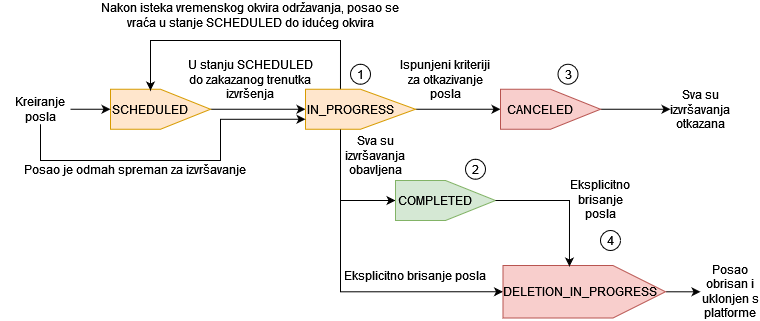
\includegraphics[scale=0.5]{imgs/job_states}
	\caption{Različita stanja tijekom izvršavanja posla \cite{aws_docs}}
	\label{fig:job_states}
\end{figure}

Postoje određena ograničenja na poslove i njihovo izvršavanje. Svi poslovi u stanju \textit{IN\_PROGRESS} smatraju se aktivnim poslovima za koje postoji limit. Ovo uključuje poslove koji ili uvode nova izvršavanja poslova ili poslove koji čekaju da uređaji dovrše postojeće izvršavanje. Ograničenje se odnosi na kontinuirane i jednokratne poslove. Poslovi u tijeku i poslovi koji poništavaju izvršenja prethodno stvorenih poslova istovremeni su i ubrajaju se u ograničenje istovremenosti poslova. Usluga može pokretati i otkazivati izvršenje poslova brzinom od tisuću uređaja u minuti. Svaki posao je istovremen i ubraja se u ograničenje istovremenosti poslova samo kratko vrijeme. Nakon što su izvršenja uvedena ili otkazana, posao više nije istovremen i ne ubraja se u ograničenje istovremenosti poslova. Moguće je iskoristiti istovremenost za kreiranje većeg broja poslova za vrijeme čekanja izvršenja postojećih poslova.

Isto tako, postoje različita stanja izvršenja samog posla. Izvršenje posla odnosi se na jednu instancu pokretanja posla na određenom ciljnom uređaju, te skup svih izvršenja poslova na svim uređajima određuje stanje samog posla. Tablica \ref{table:job_exec_states} prikazuje sva stanja u kojima se može naći izvršenje nekog posla. Isto tako, u tablici je navedeno koje stanje može okinuti uređaj, a koje usluga. Označeno je i koja su stanja prekidna, odnosno označavaju završetak izvođenja posla. Stupac \textit{retry} odnosi se na mogućnost ponovnog pokušaja izvršenja posla nakon navedenog stanja. 

\begin{table}[ht!]
	\centering
	\caption{Stanja izvršenja posla \cite{aws_docs}}
	\begin{tabular}{|c| c| c| c| c|}
		\hline
		\rowcolor{lightblue}  
		\textbf{Stanje} & \textbf{Pokrenuo uređaj?} & \textbf{Pokrenula usluga?} & \textbf{Prekidno?} & \textbf{\textit{Retry}?} \\ \hline
		\textit{QUEUED} & Ne & Da & Ne & - \\ \hline
		\textit{IN\_PROGRESS} & Da & Ne & Ne & - \\ \hline
		\textit{SUCCEEDED} & Da & Ne & Da & - \\ \hline
		\textit{FAILED} & Da & Ne & Da & Da \\ \hline
		\textit{TIMED\_OUT} & Ne & Da & Da & Da \\ \hline
		\textit{REJECTED} & Da & Ne & Da & Ne \\ \hline
		\textit{REMOVED} & Ne & Da & Da & Ne \\ \hline
		\textit{CANCELED} & Ne & Da & Da & Ne \\ \hline
	\end{tabular}
	\label{table:job_exec_states}
\end{table}

Kad usluga pošalje posao na ciljni uređaj, status izvršenja posla prelazi u \textit{QUEUED}. Posao stoji u stanju čekanja u redu sve dok uređaj ne primi izvršenje posla, pokrene ga i promijeni status u \textit{IN\_PROGRESS} koji zatim i pošalje na platformu. Isto tako, u slučaju da se posao otkaže ili se kriteriji otkazivanja posla ispune, status izvršenja posla prelazi u \textit{CANCELED}. Pri uspješnom izvršenju posla, uređaj šalje obavijest na platformu o uspješnosti, čime se status mijenja u \textit{SUCCEEDED}. Ako pak izvršenje posla bude neuspješno, prelazi u stanje \textit{FAILED} odakle ima priliku ponovnog izvršenja ako je tako naznačeno pri konfiguraciji samog posla. Stanje \textit{TIMED\_OUT} odnosi se na istek maksimalnog vremena izvođenja, i isto tako podržava mehanizam ponovnog izvršenja. Uređaj može promijeniti stanje izvršenja posla u \textit{REJECTED} ako primi nevaljan ili nekompatibilan zahtjev od platforme. Stanje \textit{REMOVED} postavlja se ako uređaj više nije podoban ili valjan za izvršenje traženog posla. 


\subsection{AWS IoT OTA}

\subsection{Ostale dostupne IoT usluge u sustavu AWS}

Uz ranije opisanu glavnu komponentu IoT Core koju nudi AWS za stvaranje IoT aplikacija, u samom ekosustavu nalazi se još mogućnosti za jednostavniju integraciju oblaka i fizičkih uređaja. U nastavku su ukratko opisane ostale usluge koje se mogu integrirati uz jezgrenu uslugu AWS IoT Core.

Važno je napomenuti kako nisu sve usluge dostupne u svim regijama unutar platforme AWS.

\subsubsection{IoT Analytics}

AWS IoT Analytics automatizira korake potrebne za analizu podataka prikupljenih od IoT uređajima. Filtrira, transformira i obogaćuje podatke prije nego ih pohrani u vremensku bazu podataka za daljnju analizu. Moguće je postaviti uslugu da prikuplja podatke s uređaja samo koji su potrebni, vrši matematičke operacije i dopunjava podatke raznim metapodacima, primjerice o lokaciji. Zatim se podaci mogu analizirati koristeći ugrađeni sustav za pretraživanje koji koristi SQL sintaksu ili pak vršiti kompleksniju analizu koristeći usluge umjetne inteligencije. Isto tako, ova usluga nudi vizualizaciju podataka integracijom s dodatnom uslugom Amazon QuickSight. 

\subsubsection{IoT Device Defender}

AWS IoT Device Defender potpuna je usluga koja pomaže pri osiguranju IoT uređaja. Kontinuirano revidira IoT konfiguracije radi provjere jesu li sve u skladu s najboljim sigurnosnim praksama. Također pruža kontinuirano monitoriranje sigurnosnih metrika s uređaja i usluge AWS IoT Core kako bi se detektirale anomalije u ponašanju pojedinih uređaja. 

Ova usluga također omogućuje slanje alarma na konzolu AWS IoT sustava i na uslugu za monitoriranje Amazon CloudWatch. Koriste se ugrađene mitigacijske akcije kako bi se izolirali nesigurni uređaji.

\subsubsection{IoT Events}

AWS IoT Events usluga služi za praćenje događaja u sustavu. Ova usluga prati ulazne podatke s više IoT uređaja i aplikacija radi prepoznavanja uzoraka i pokretanja prikladnih operacija na određene događaje. Moguće je pratiti ne samo fizičke uređaje, nego i druge AWS aplikacije integrirane u IoT sustav.

\subsubsection{IoT FleetWise}

AWS IoT FleetWise jest usluga koja se koristi za prikupljanje podataka od vozila i njihovu organizaciju u oblaku. Prikupljeni se podaci mogu koristiti za poboljšanje kvalitete, performansa i autonomije vozila. Također podržava više različitih protokola i podatkovnih formata. Ova usluga pomaže pri transformaciji poruka niske razine \engl{low-level} u oblik čitljiv čovjeku i standardizira podatke radi lakše analize u oblaku. Moguće je također definirati vrstu podataka i trenutak u kojem se ti podaci šalju u oblak.

Kada su podaci o vozilu u oblaku, mogu se koristiti u aplikacijama koje analiziraju zdravlje vozila. Ove informacije mogu pomoći pri identifikaciji potencijalnih problema u održavanju i pri unapređenju naprednih tehnologija poput autonomne i asistirane vožnje integracijom strojnog učenja.

\subsubsection{IoT Greengrass}

AWS IoT Greengrass jest usluga otvorenog koda \engl{open source} za računarstvo na rubu \engl{edge computing} i u oblaku koja pomaže pri izradi, objavi i upravljanju IoT aplikacija na uređajima. Može se koristiti za omogućavanje uređajima lokalno reagiranje na podatke koje generiraju, pokretanje modela strojnog učenja za predikciju, te filtriranje i agregaciju podataka s uređaja. Omogućava uređajima da prikupljaju i analiziraju podatke ne u oblaku, nego ili na samom uređaju ili drugom mjestu koje je bliže izvorištu tih podataka. Također može komunicirati na siguran način s uslugom AWS IoT Core i izvoziti podatke u oblak. Karakteristika računarstva u rubu, koje omogućava ova komponenta, jest približavanje računanja izvorišnim uređajima, čime se poboljšava vrijeme odziva i štedi propusnost \cite{what_is_edge}.

\subsubsection{IoT Roborunner}

AWS IoT RoboRunner nova je usluga koja pruža infrastrukturu za optimizaciju robota iz jedne točke gledišta. Uz pomoć ove usluge moguće je izgraditi aplikacije za jednostavniji međusobni rad robota. Namijenjena je za industrijske robote i automatizirane sustave za olakšano upravljanje opremom. Pruža centralne repozitorije podataka za pohranu te podržava različite podatkovne formate od raznih robota i autonomnih sustava.

\subsubsection{IoT TwinMaker}

AWS IoT TwinMaker usluga je za kreiranje operativnih digitalnih dvojnika fizičkih i digitalnih sustava. Stvara digitalne vizualizacije koristeći mjerenja i analize iz raznih senzora i kamera radi praćenja stvarnog stanja i uvjeta u kojima se objekt, zgrada ili kompleks nalazi. Podaci iz stvarnog svijeta se mogu koristiti za dijagnostiku i ispravljanje pogrešaka ili pak optimizaciju operacija. 

Digitalni dvojnik \engl{digital twin} digitalna je reprezentacija sustava i svih njegovih fizičkih i digitalnih komponenti. Dinamički se ažurira primitkom novih podataka kako bi simulirao stvarno stanje i ponašanje sustava. 


\subsubsection{IoT SiteWise}

AWS IoT SiteWise jest usluga koja skalabilno prikuplja, modelira, analizira i vizualizira podatke iz industrijske opreme. Usluga pruža kreiranje web aplikacija za operativne korisnike radi prikaza i analize industrijskih podataka u stvarnom vremenu. Moguće je dobiti uvide u podatke i operacije konfiguriranjem i praćenjem raznih metrika, primjerice efektivnost i efikasnost opreme. Ovu je uslugu moguće koristiti jedino uz ranije opisan IoT TwinMaker.

\eject